\documentclass{beamer}
\usepackage{graphicx}
\usepackage{amsmath}

\title{Detailed Explanations of Fiscal Policy Concepts}
\author{Charles Ancel}
\date{July 24, 2024}

\begin{document}

\frame{\titlepage}

\section{Introduction}
\begin{frame}
    \frametitle{Introduction}
    My name is Charles Ancel, my UIN is 654604114, and this is my ID. I'm currently enrolled in ECON 425 during the Summer Session. This assignment is part of the requirement from the University regarding the College of LAS's identity verification policy for LAS Online-certified classes. For the answers in this assignment, I did not use any form of Artificial Intelligence (AI) help, such as Chat-GPT or similar, and thus my answers will accurately and fairly reflect my own learning from this course.
\end{frame}

\begin{frame}
    \frametitle{Scenario Context}
    Imagine a debate with someone who disregards economic theory and challenges the standard theories behind fiscal policy. This presentation addresses their questions and statements using the knowledge gained from ECON 425, specifically chapter 7.
\end{frame}

\section{Ricardian Equivalence}
\begin{frame}
    \frametitle{Ricardian Equivalence}
    \textbf{Question 1:} I don’t believe in the Ricardian equivalence. Why should anybody care about learning such a thing? I think that it is devoid of any substance and thus I see it as a complete waste of time.
    
    \textbf{Explanation:} Ricardian Equivalence is an economic theory that suggests when a government increases deficit spending, consumers anticipate higher taxes in the future to pay off the debt. As a result, they increase their savings and reduce current consumption, offsetting the increase in demand from the government spending.
    
    \textbf{Definition:} Ricardian Equivalence proposes that consumer behavior will offset government fiscal policy changes due to rational expectations.
    
    \textbf{Real-World Example:} Consider a government that issues bonds to finance a stimulus package. According to Ricardian Equivalence, consumers might save money to prepare for future tax increases required to repay the bonds, thus neutralizing the stimulus effect.
\end{frame}

\begin{frame}
    \frametitle{Importance of Ricardian Equivalence}
    Ricardian Equivalence is crucial for understanding the long-term effects of government borrowing. It helps economists and policymakers analyze how consumers might react to changes in fiscal policy by saving more in anticipation of future tax burdens. This theory underscores the importance of considering future tax implications when implementing debt-financed policies, providing insights into consumer behavior and fiscal responsibility.
\end{frame}

\begin{frame}
    \frametitle{Diagram of Ricardian Equivalence}
    \begin{figure}[h!]
        \centering
        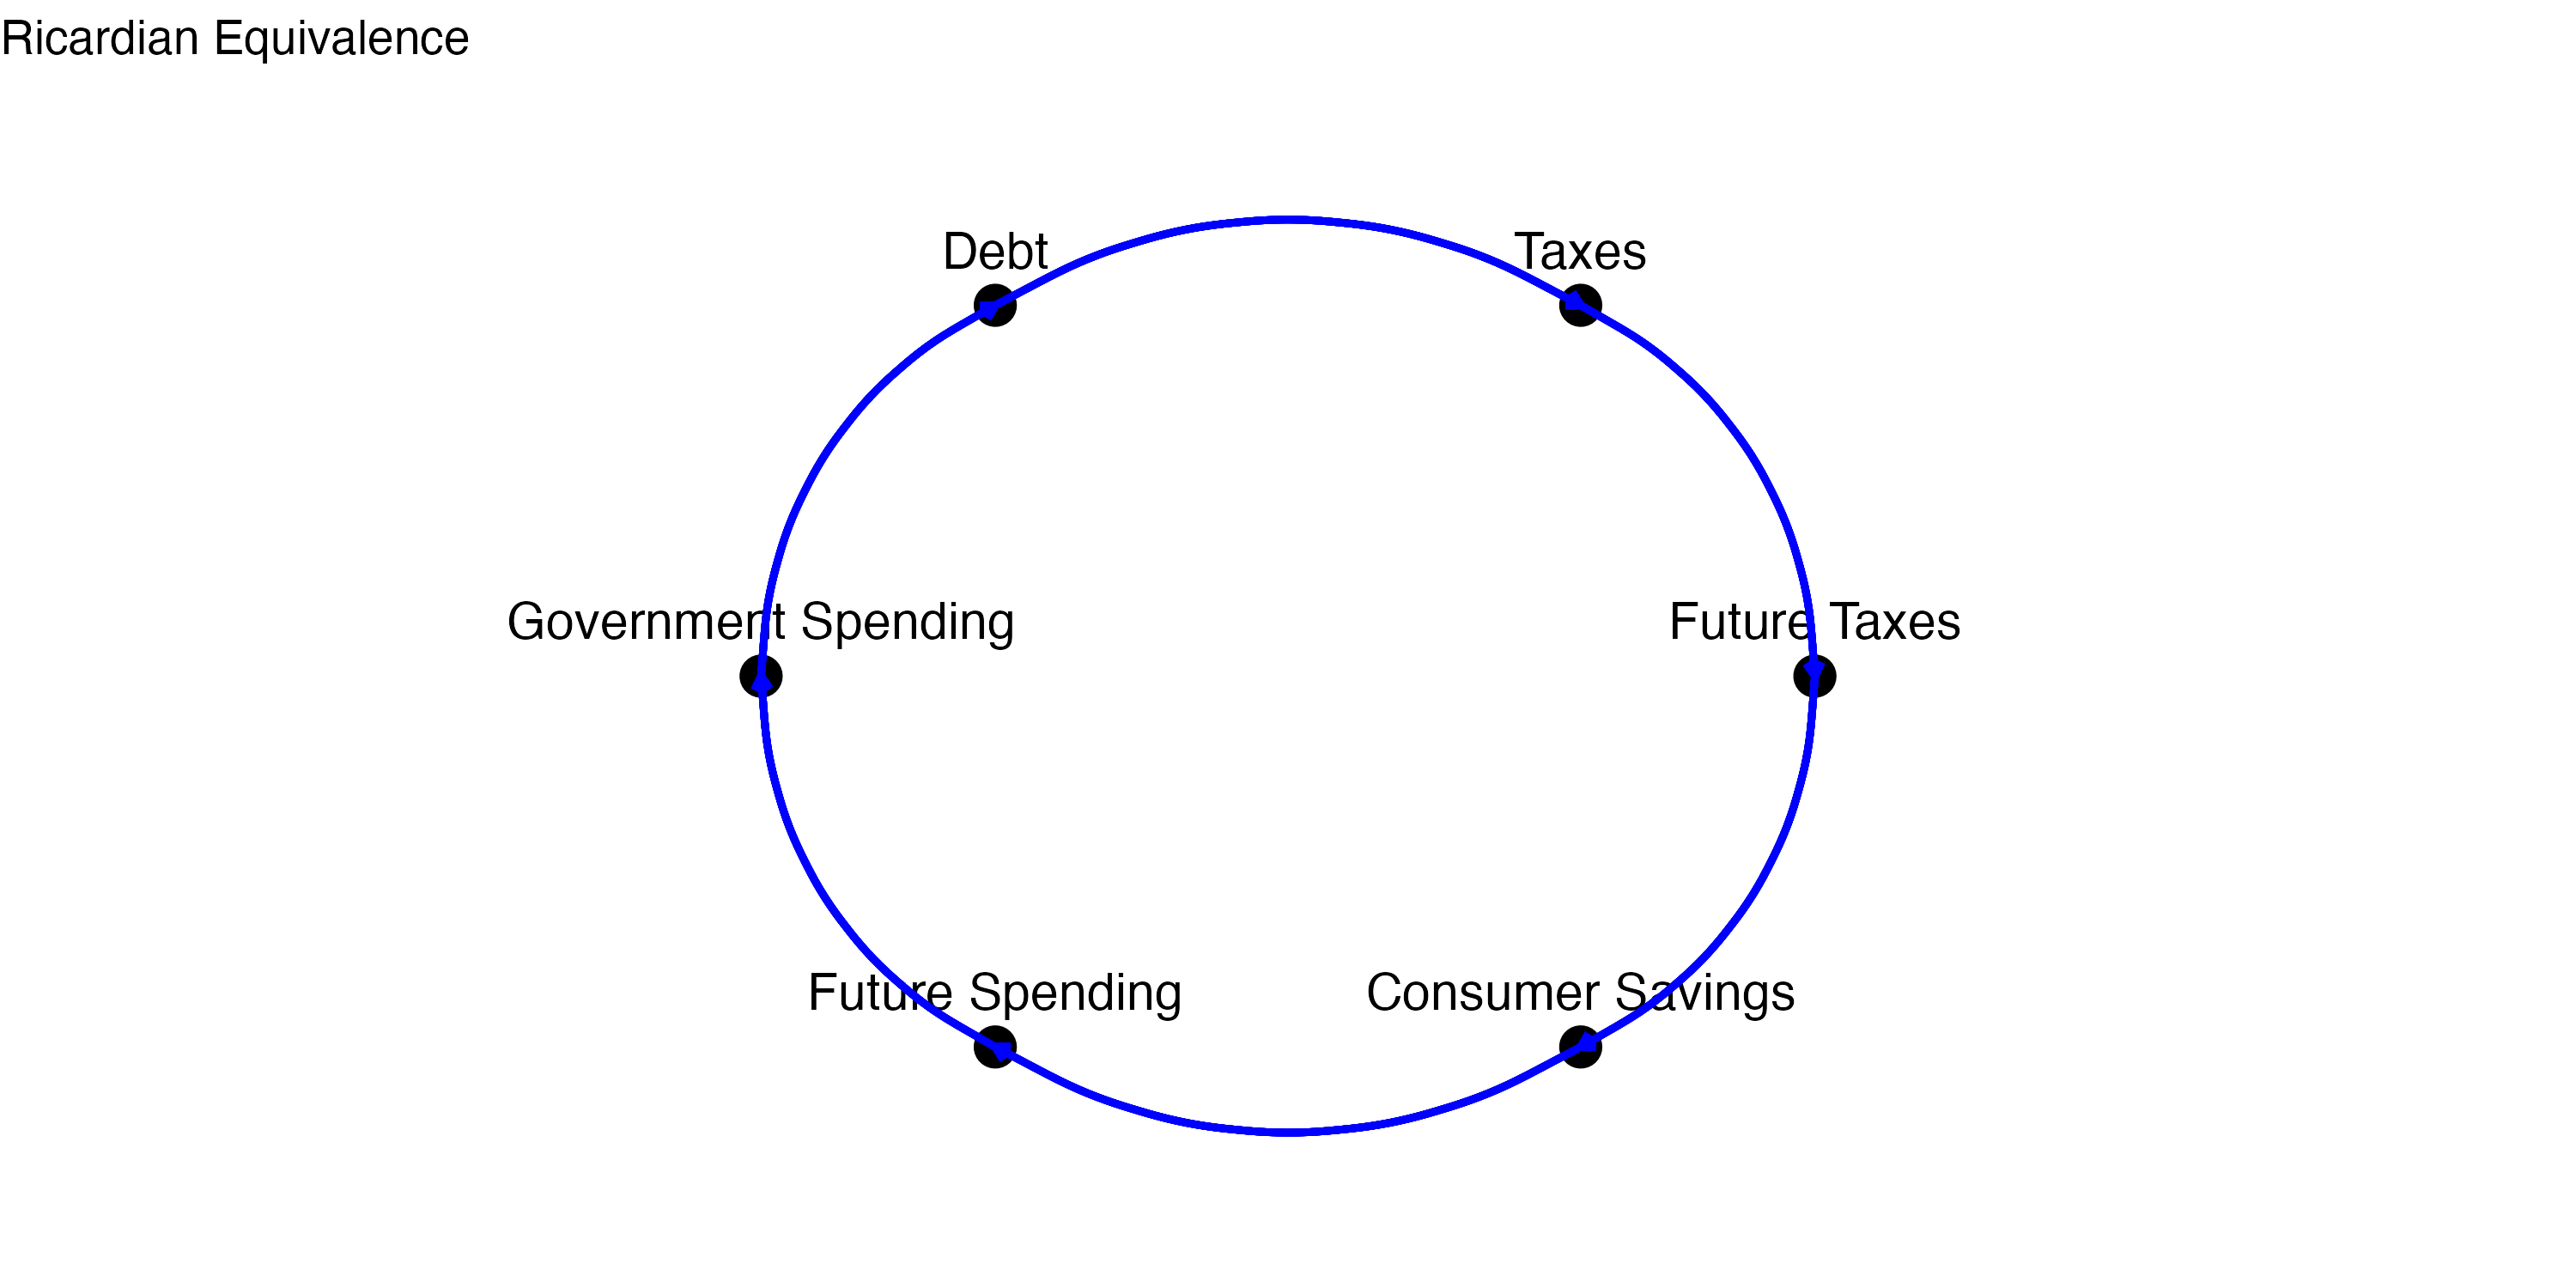
\includegraphics[width=0.8\textwidth]{/Users/cancel/Personal/Coursework/Econ425/VA3/R/Ricardian_Equivalence.png}
        \caption{Diagram of Ricardian Equivalence}
    \end{figure}
\end{frame}

\begin{frame}
    \frametitle{Graph Explanation: Ricardian Equivalence}
    This diagram illustrates the relationship between government spending, debt, taxes, and consumer savings. It shows how government borrowing can lead to future taxes, affecting consumer savings and consumption.
\end{frame}

\begin{frame}
    \frametitle{Key Takeaways: Ricardian Equivalence}
    Understanding Ricardian Equivalence helps in predicting consumer behavior in response to fiscal policy, emphasizing the significance of future tax burdens in policy decisions. Although it is a theoretical concept, it provides a framework for analyzing the potential long-term impacts of government borrowing on the economy.
\end{frame}

\section{Government Deficit and Constraints}
\begin{frame}
    \frametitle{Government Deficit and Constraints}
    \textbf{Question 2:} I’ve read this book written by a Twitter celebrity that says the government can increase its deficit forever without any actual constraint. Why is the government not doing that already?

    \textbf{Explanation:} While increasing the government deficit can stimulate the economy in the short run, continuously increasing the deficit can lead to higher interest rates and inflation, crowding out private investment and reducing economic growth. Sustainable fiscal policy is crucial for long-term economic stability. Moreover, unchecked deficits can undermine market confidence and lead to a sovereign debt crisis.

    \textbf{Definition:} A government deficit occurs when expenditures exceed revenues, necessitating borrowing to finance the shortfall.

    \textbf{Real-World Example:} The Eurozone crisis, where countries like Greece faced severe financial instability due to unsustainable deficits and debt levels.
\end{frame}

\begin{frame}
    \frametitle{Government Debt and Interest Rate}
    \begin{figure}[h!]
        \centering
        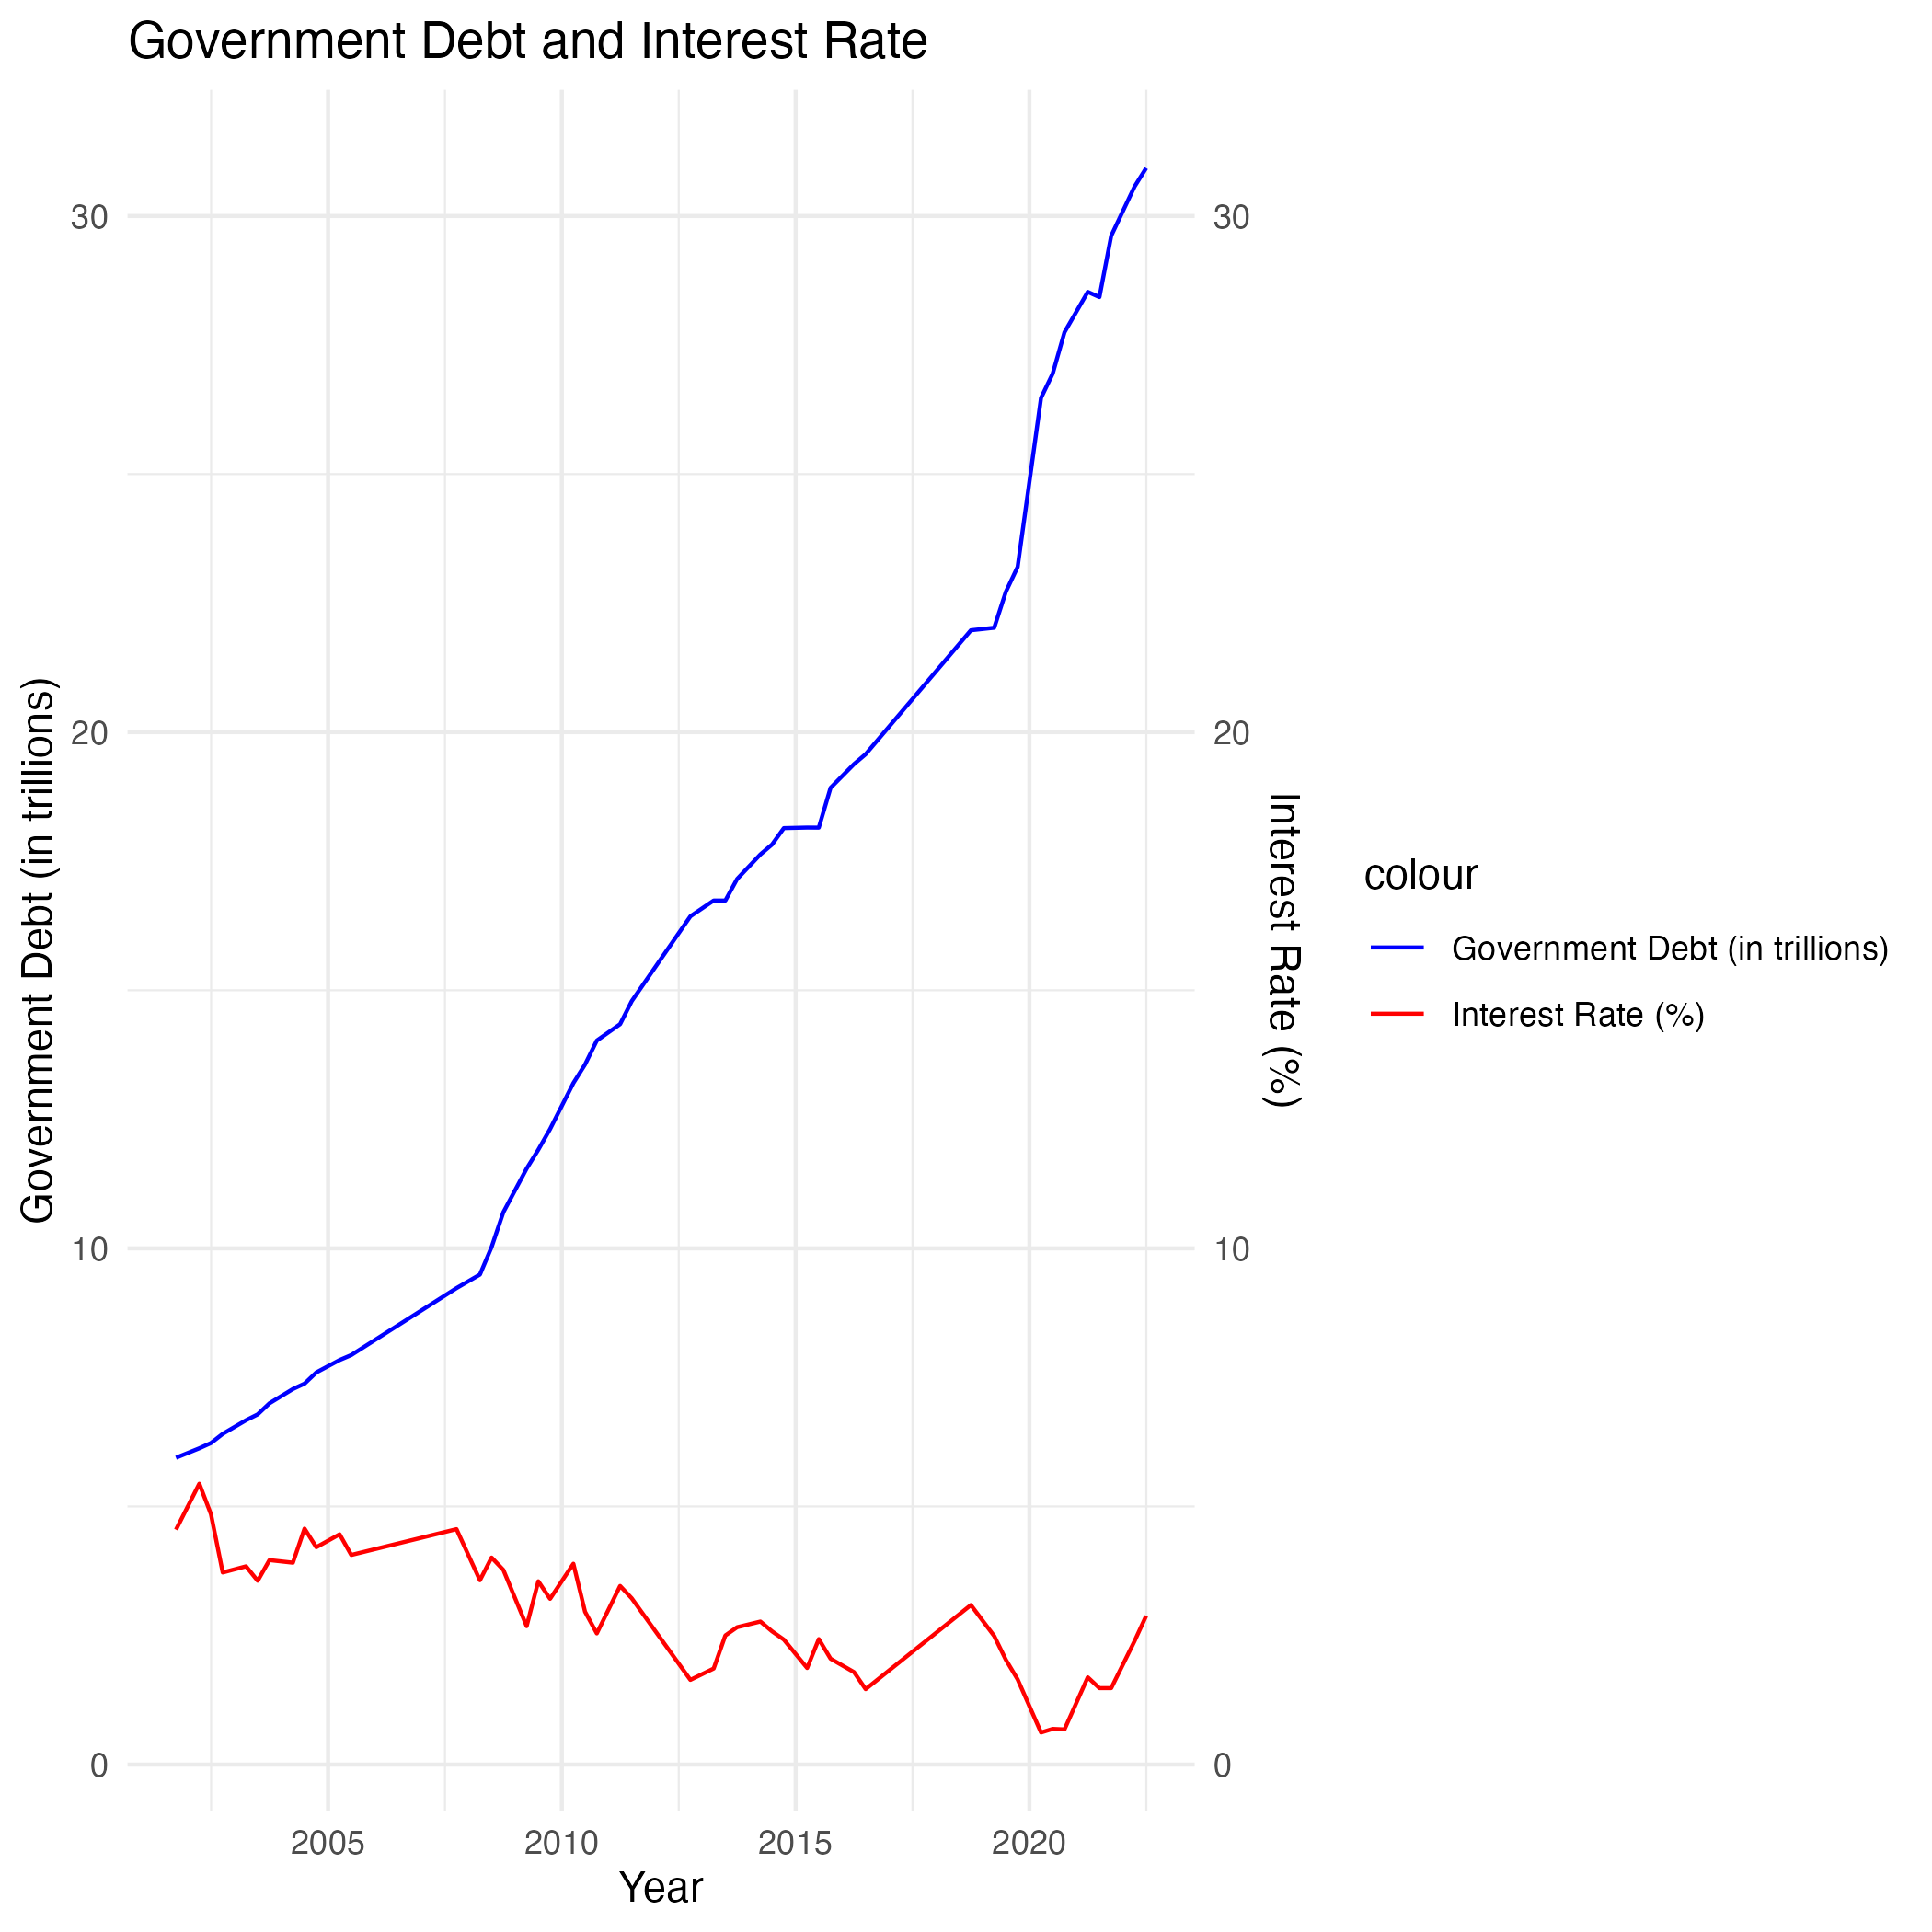
\includegraphics[width=0.8\textwidth]{/Users/cancel/Personal/Coursework/Econ425/VA3/R/Debt_Constraints.png}
        \caption{Government Debt and Interest Rate}
    \end{figure}
\end{frame}

\begin{frame}
    \frametitle{Graph Explanation: Government Debt and Interest Rate}
    This plot shows the relationship between government debt and interest rates. It demonstrates how rising government debt can lead to higher interest rates, which can negatively impact economic growth by increasing the cost of borrowing for both the government and the private sector.
\end{frame}

\begin{frame}
    \frametitle{Key Takeaways: Government Deficit and Constraints}
    Continuous deficits can lead to unsustainable debt levels, causing inflation and higher interest rates. Maintaining market confidence is essential for stable borrowing costs. Understanding these constraints helps in designing sustainable fiscal policies that balance short-term economic stimulation with long-term financial stability.
\end{frame}

\section{General Equilibrium Models}
\begin{frame}
    \frametitle{General Equilibrium Models}
    \textbf{Question 3:} General equilibrium models are not helpful to understand fiscal policy because they are too simplistic. The real world is at odds with such models. Furthermore, with the Big Data availability that we have now, models are no longer required.

    \textbf{Explanation:} General equilibrium models, while simplified, provide a framework to understand the interactions between different sectors of the economy. They help predict the effects of policy changes on the economy. Big Data can enhance these models but cannot replace the theoretical framework they provide. Models are essential for isolating specific variables and understanding causal relationships, which is crucial for policy analysis.

    \textbf{Definition:} General equilibrium models examine the simultaneous equilibrium in multiple markets and their interactions.

    \textbf{Real-World Example:} Using a computable general equilibrium (CGE) model to assess the impact of a carbon tax on different industries and the overall economy.
\end{frame}

\begin{frame}
    \frametitle{General Equilibrium Model}
    \begin{figure}[h!]
        \centering
        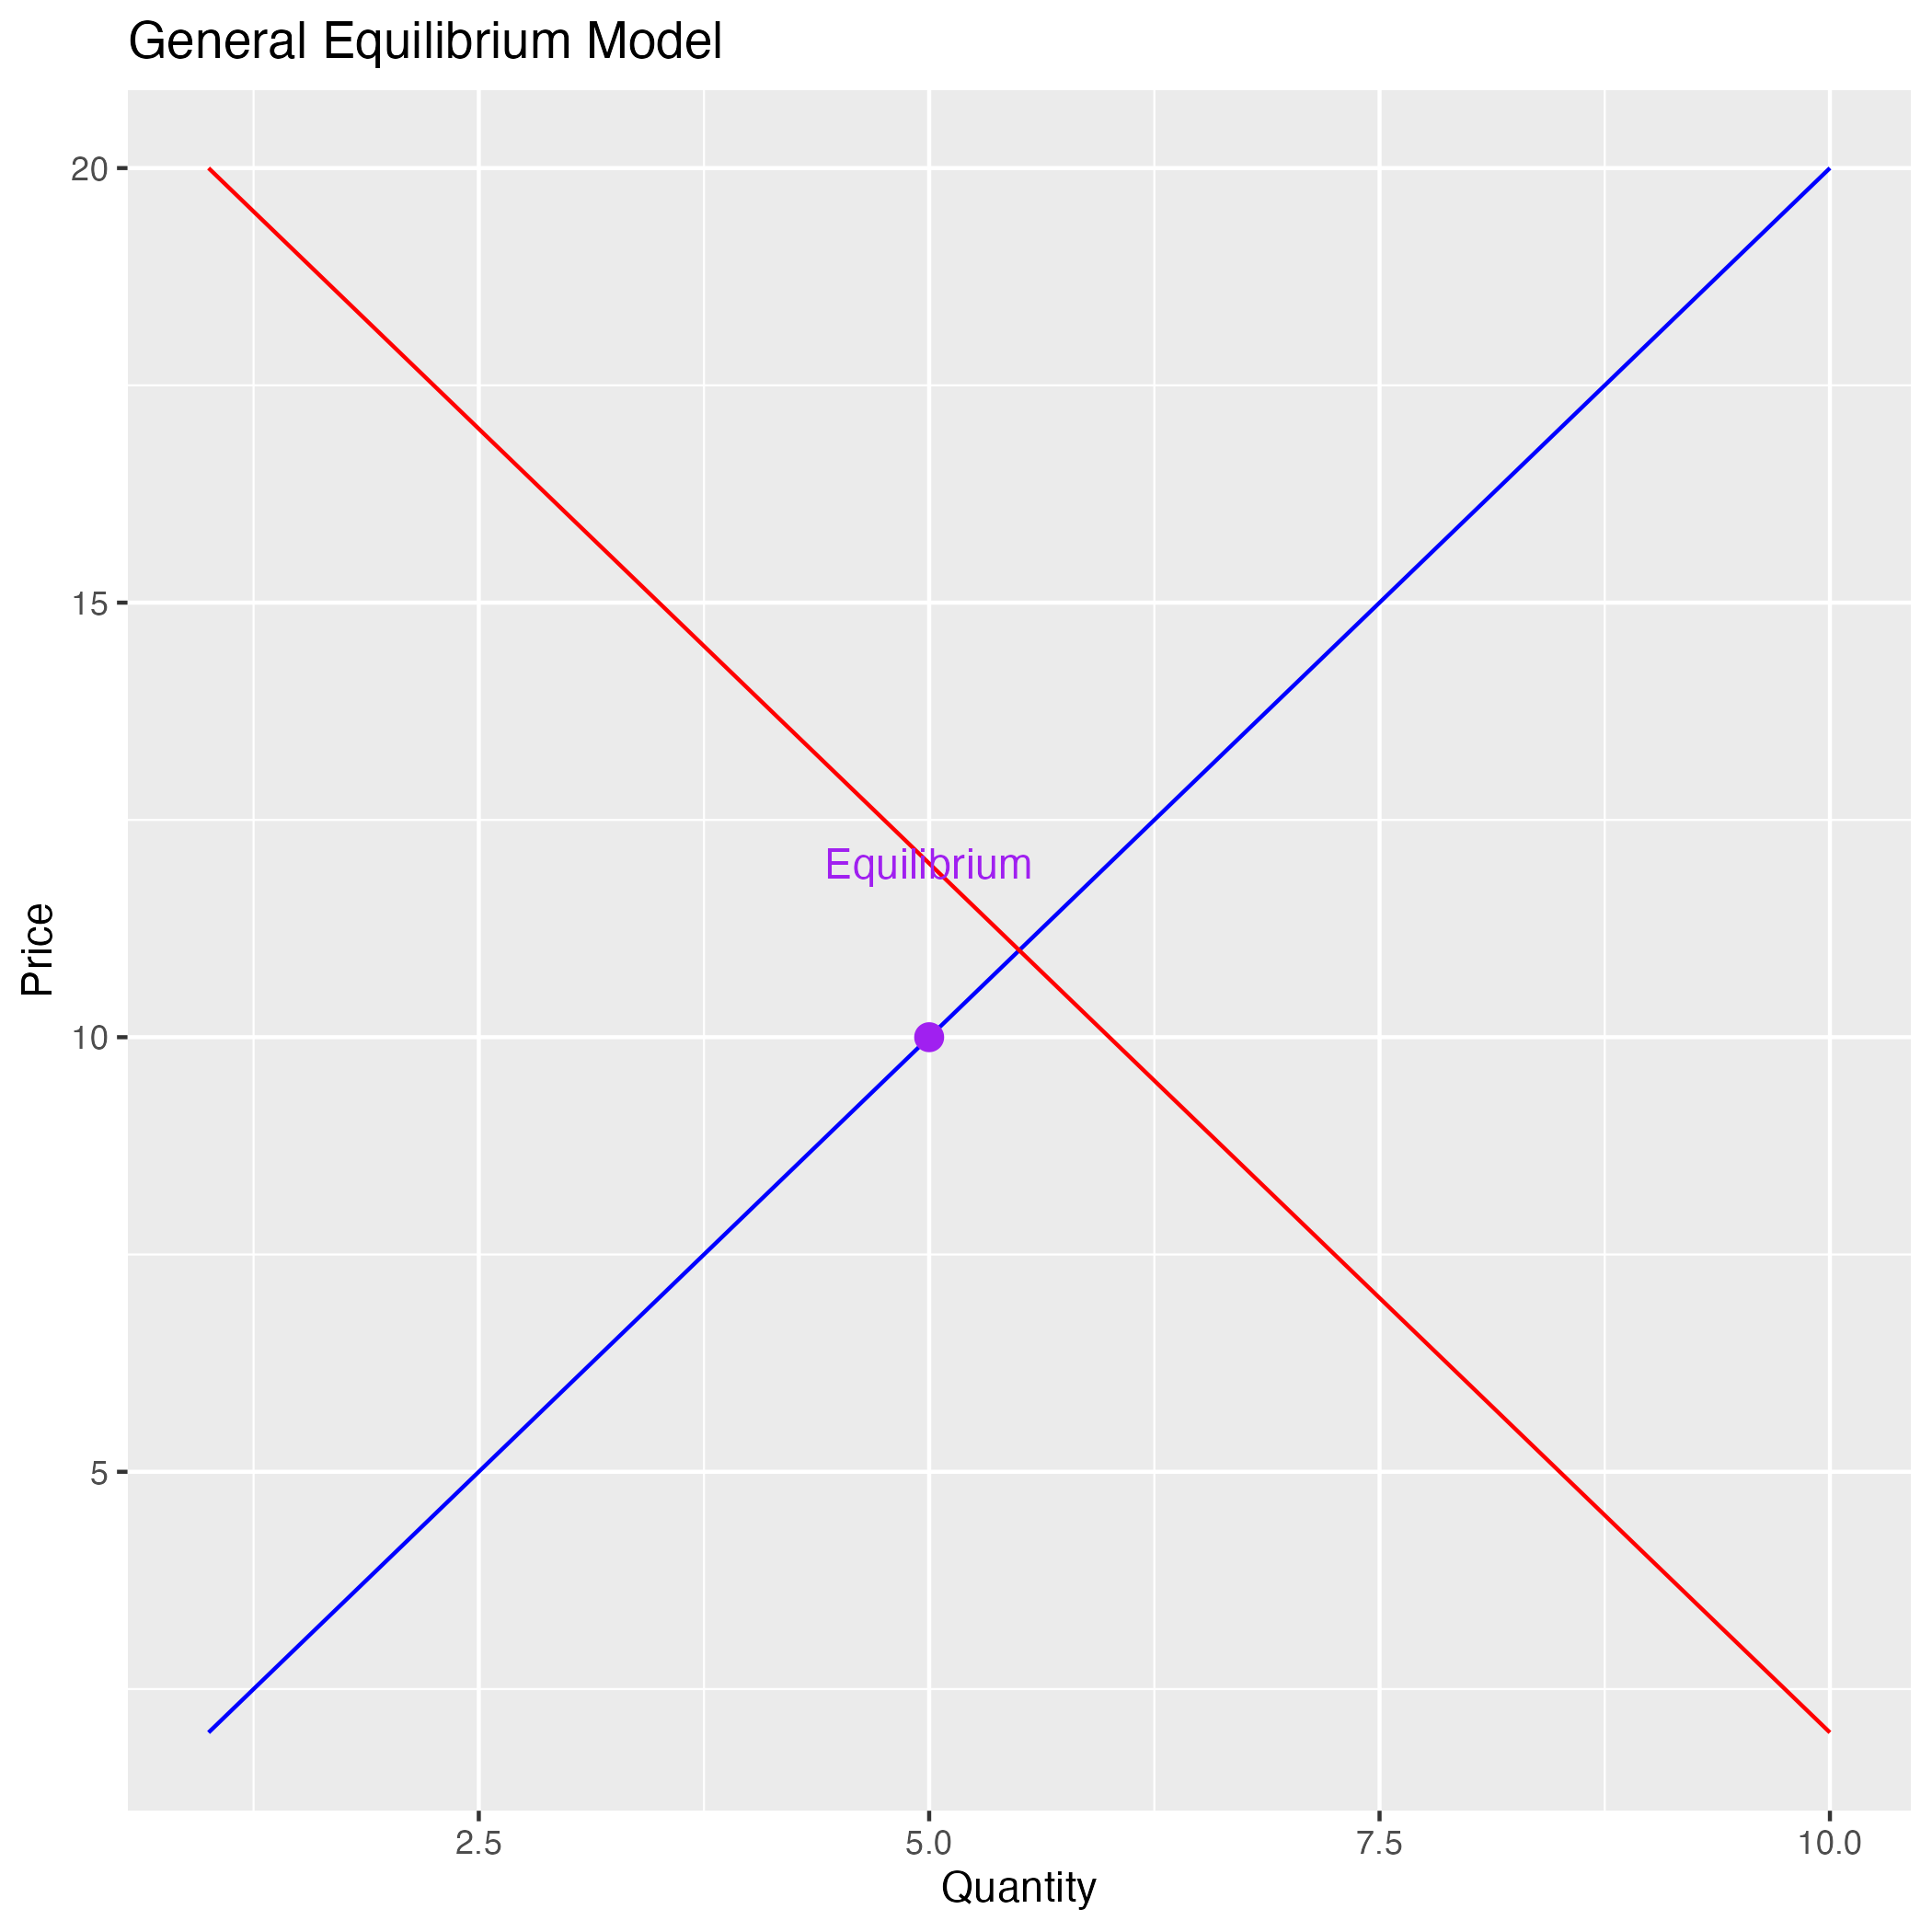
\includegraphics[width=0.8\textwidth]{/Users/cancel/Personal/Coursework/Econ425/VA3/R/General_Equilibrium.png}
        \caption{General Equilibrium Model}
    \end{figure}
\end{frame}

\begin{frame}
    \frametitle{Graph Explanation: General Equilibrium Model}
    This plot shows the equilibrium point in a simple supply and demand model, representing how markets balance out over time. It helps illustrate the foundational principles of how markets operate and respond to different economic policies.
\end{frame}

\begin{frame}
    \frametitle{Key Takeaways: General Equilibrium Models}
    General equilibrium models provide a structured way to analyze economic interactions and predict potential impacts of policy changes. While Big Data enhances model accuracy, theoretical models remain essential for understanding causal relationships and informing policy analysis.
\end{frame}

\section{Government Spending Multiplier}
\begin{frame}
    \frametitle{Government Spending Multiplier}
    \textbf{Question 4:} I don’t know why you say that the government spending multiplier is around 0.7 to 1.2. I read a piece of news that reported fiscal multipliers close to 2, and these were based on modern empirical research. Thus, we should fight for fiscal policies that push for the greatest government spending ever. Don’t you think?

    \textbf{Explanation:} The government spending multiplier measures the impact of government spending on GDP. Estimates of the multiplier can vary depending on the economic conditions and methodology used in the studies. The value of the multiplier is often higher during periods of economic slack or recession and lower during periods of full employment. It is essential to consider the context in which these multipliers are estimated to avoid overestimating the impact of fiscal policies.

    \textbf{Definition:} The government spending multiplier is the ratio of a change in national income to the change in government spending that causes it.

    \textbf{Real-World Example:} During the 2008 financial crisis, many studies estimated the fiscal multipliers for the stimulus packages implemented by various governments.
\end{frame}

\begin{frame}
    \frametitle{Government Spending Multipliers}
    \begin{figure}[h!]
        \centering
        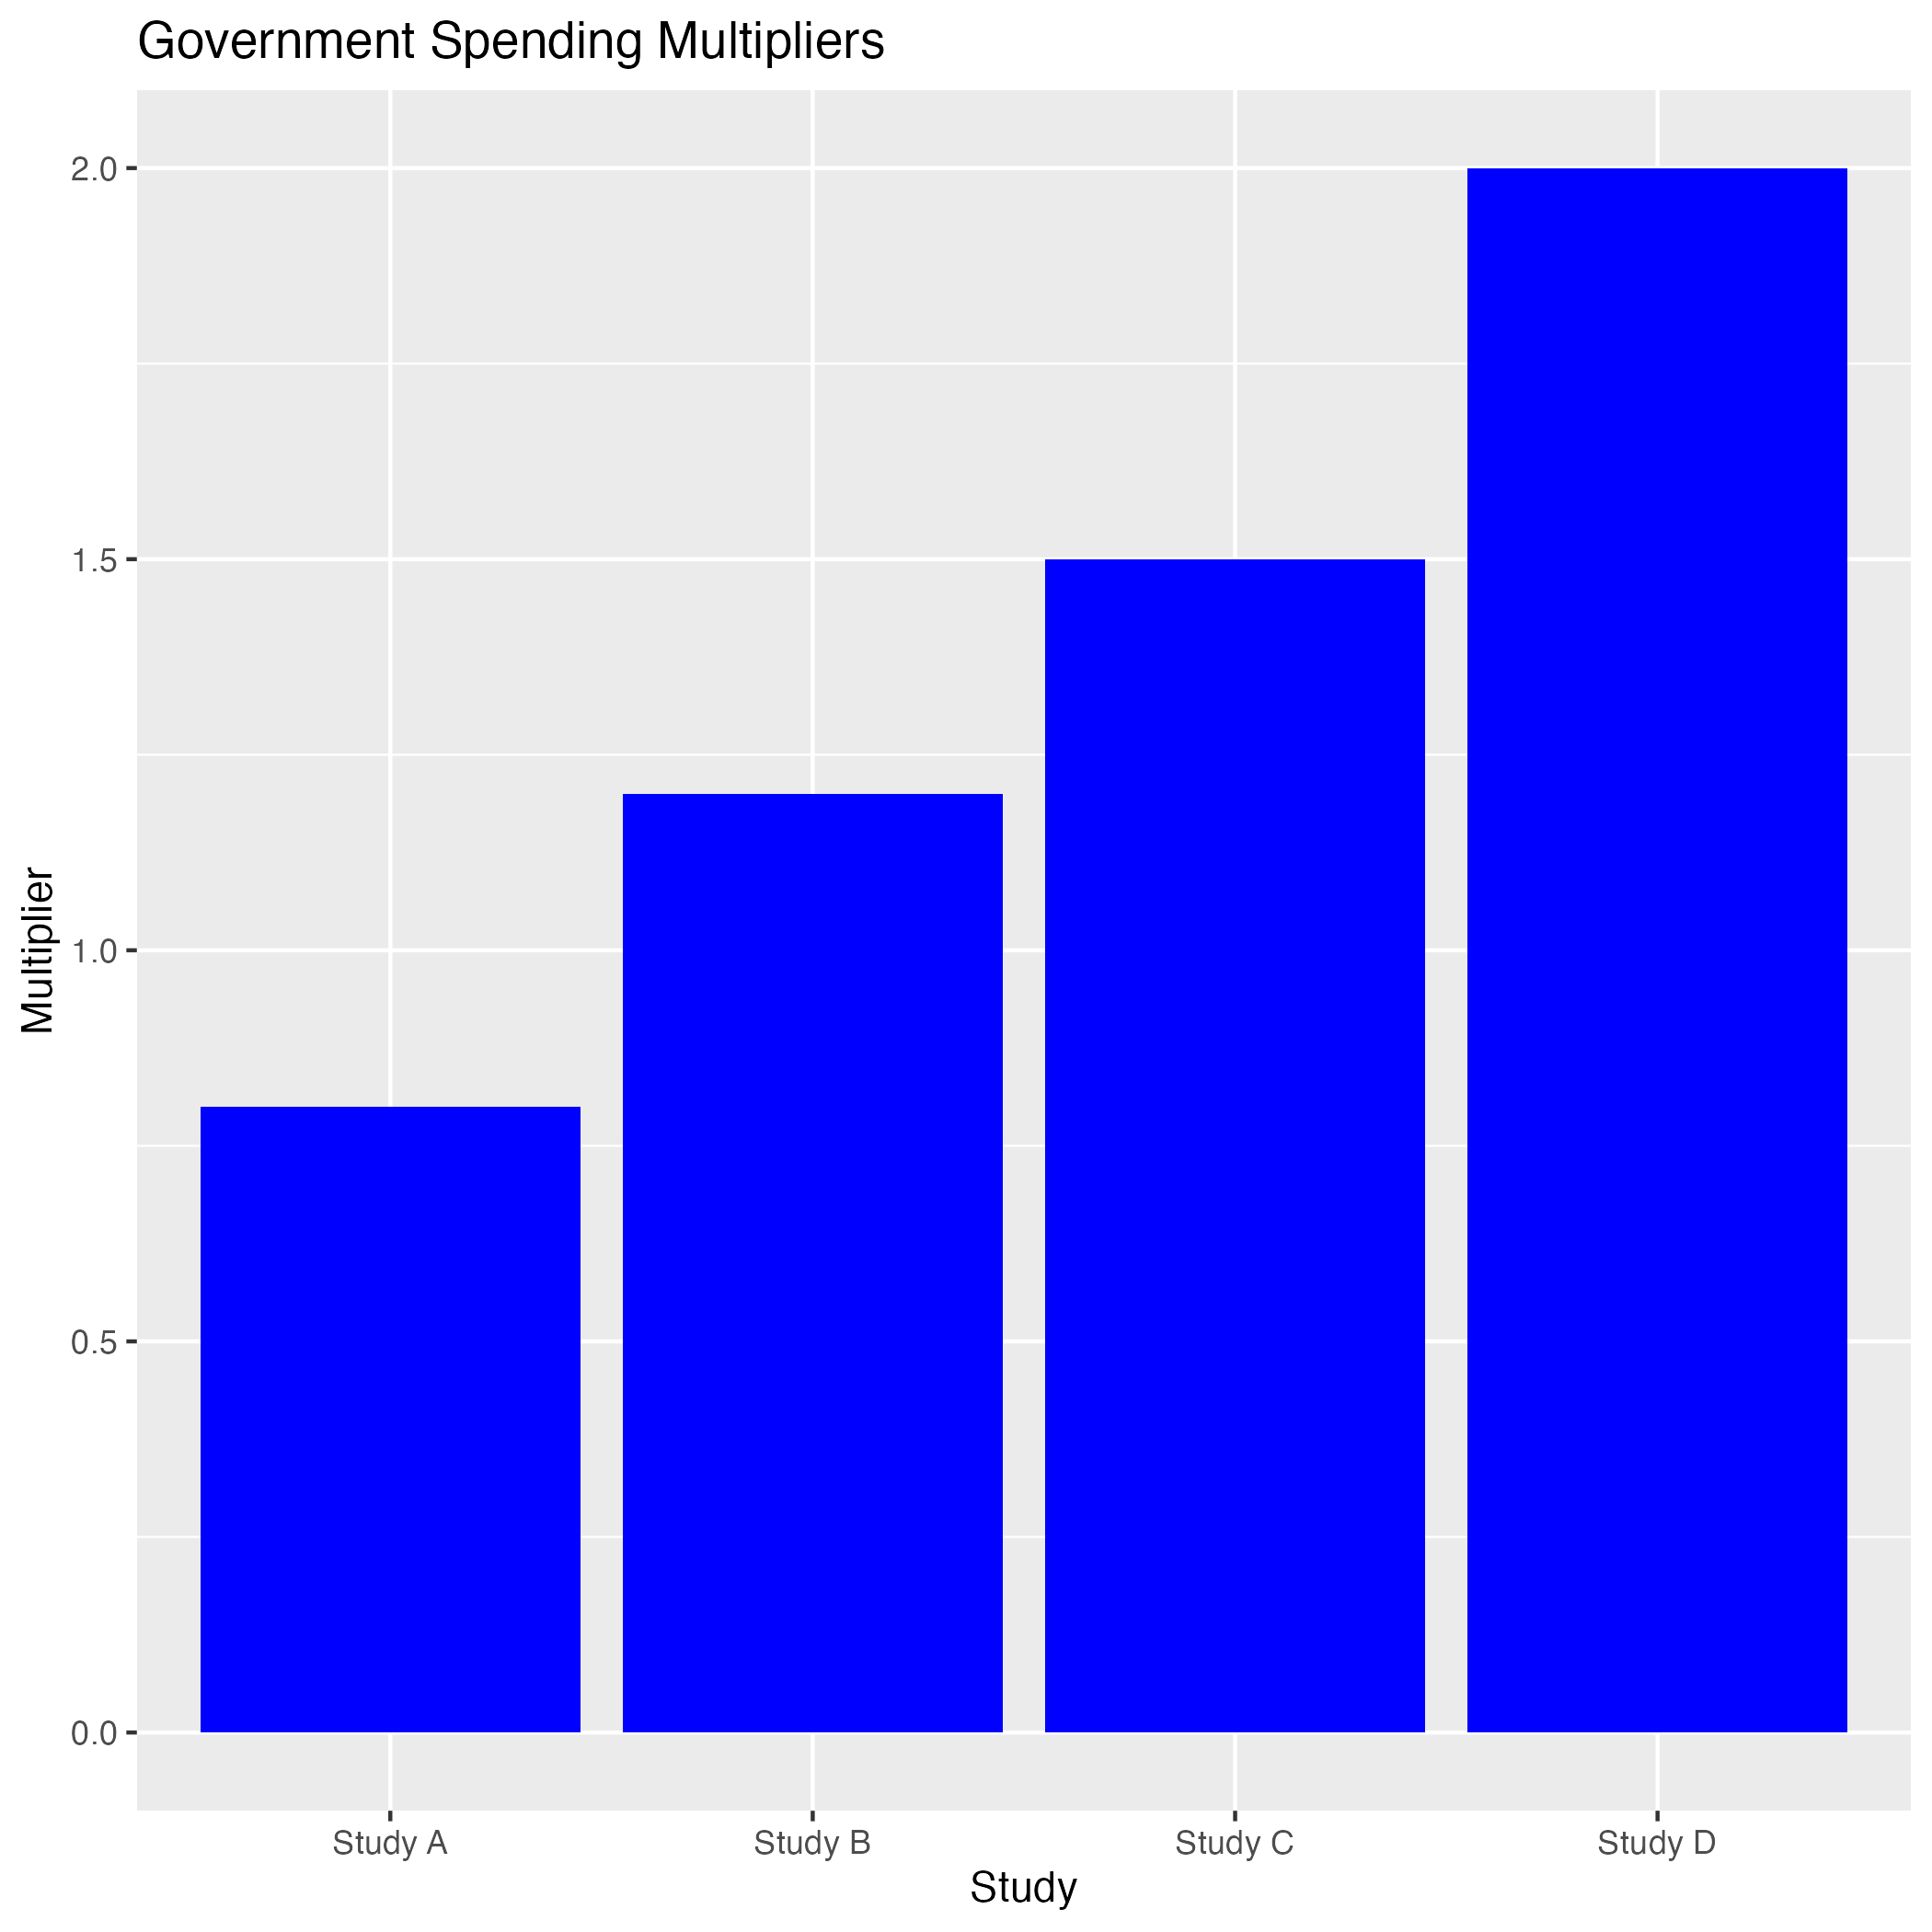
\includegraphics[width=0.8\textwidth]{/Users/cancel/Personal/Coursework/Econ425/VA3/R/Spending_Multiplier.png}
        \caption{Government Spending Multipliers}
    \end{figure}
\end{frame}

\begin{frame}
    \frametitle{Graph Explanation: Government Spending Multipliers}
    This bar plot compares different estimates of government spending multipliers from various studies, highlighting the variability in estimates and the factors influencing these values, such as the state of the economy and the type of spending.
\end{frame}

\begin{frame}
    \frametitle{Key Takeaways: Government Spending Multiplier}
    The effectiveness of government spending depends on the economic context, with higher multipliers more likely in a recession. Accurate estimation of multipliers requires considering various economic conditions to avoid overestimating the impact of fiscal policies.
\end{frame}

\section{Fiscal Multipliers and Tax Cuts}
\begin{frame}
    \frametitle{Fiscal Multipliers and Tax Cuts}
    \textbf{Question 5:} If you insist that the government spending multiplier is around 1, we still have other fiscal multipliers we can use. Surely we can implement income tax cuts that cause effects that are as strong or even stronger than what we would get with government spending.

    \textbf{Explanation:} While tax cuts can stimulate the economy, their effectiveness depends on how consumers respond. Higher-income households might save the additional income rather than spend it, leading to a lower multiplier effect compared to government spending. Additionally, the timing and structure of the tax cuts can significantly influence their impact on economic activity.

    \textbf{Definition:} The tax multiplier measures the change in GDP resulting from a change in taxes.

    \textbf{Real-World Example:} The 2001 and 2003 tax cuts in the United States aimed to stimulate economic growth but had varying impacts depending on the income levels of the recipients.
\end{frame}

\begin{frame}
    \frametitle{Fiscal Multipliers: Spending vs. Tax Cuts}
    \begin{figure}[h!]
        \centering
        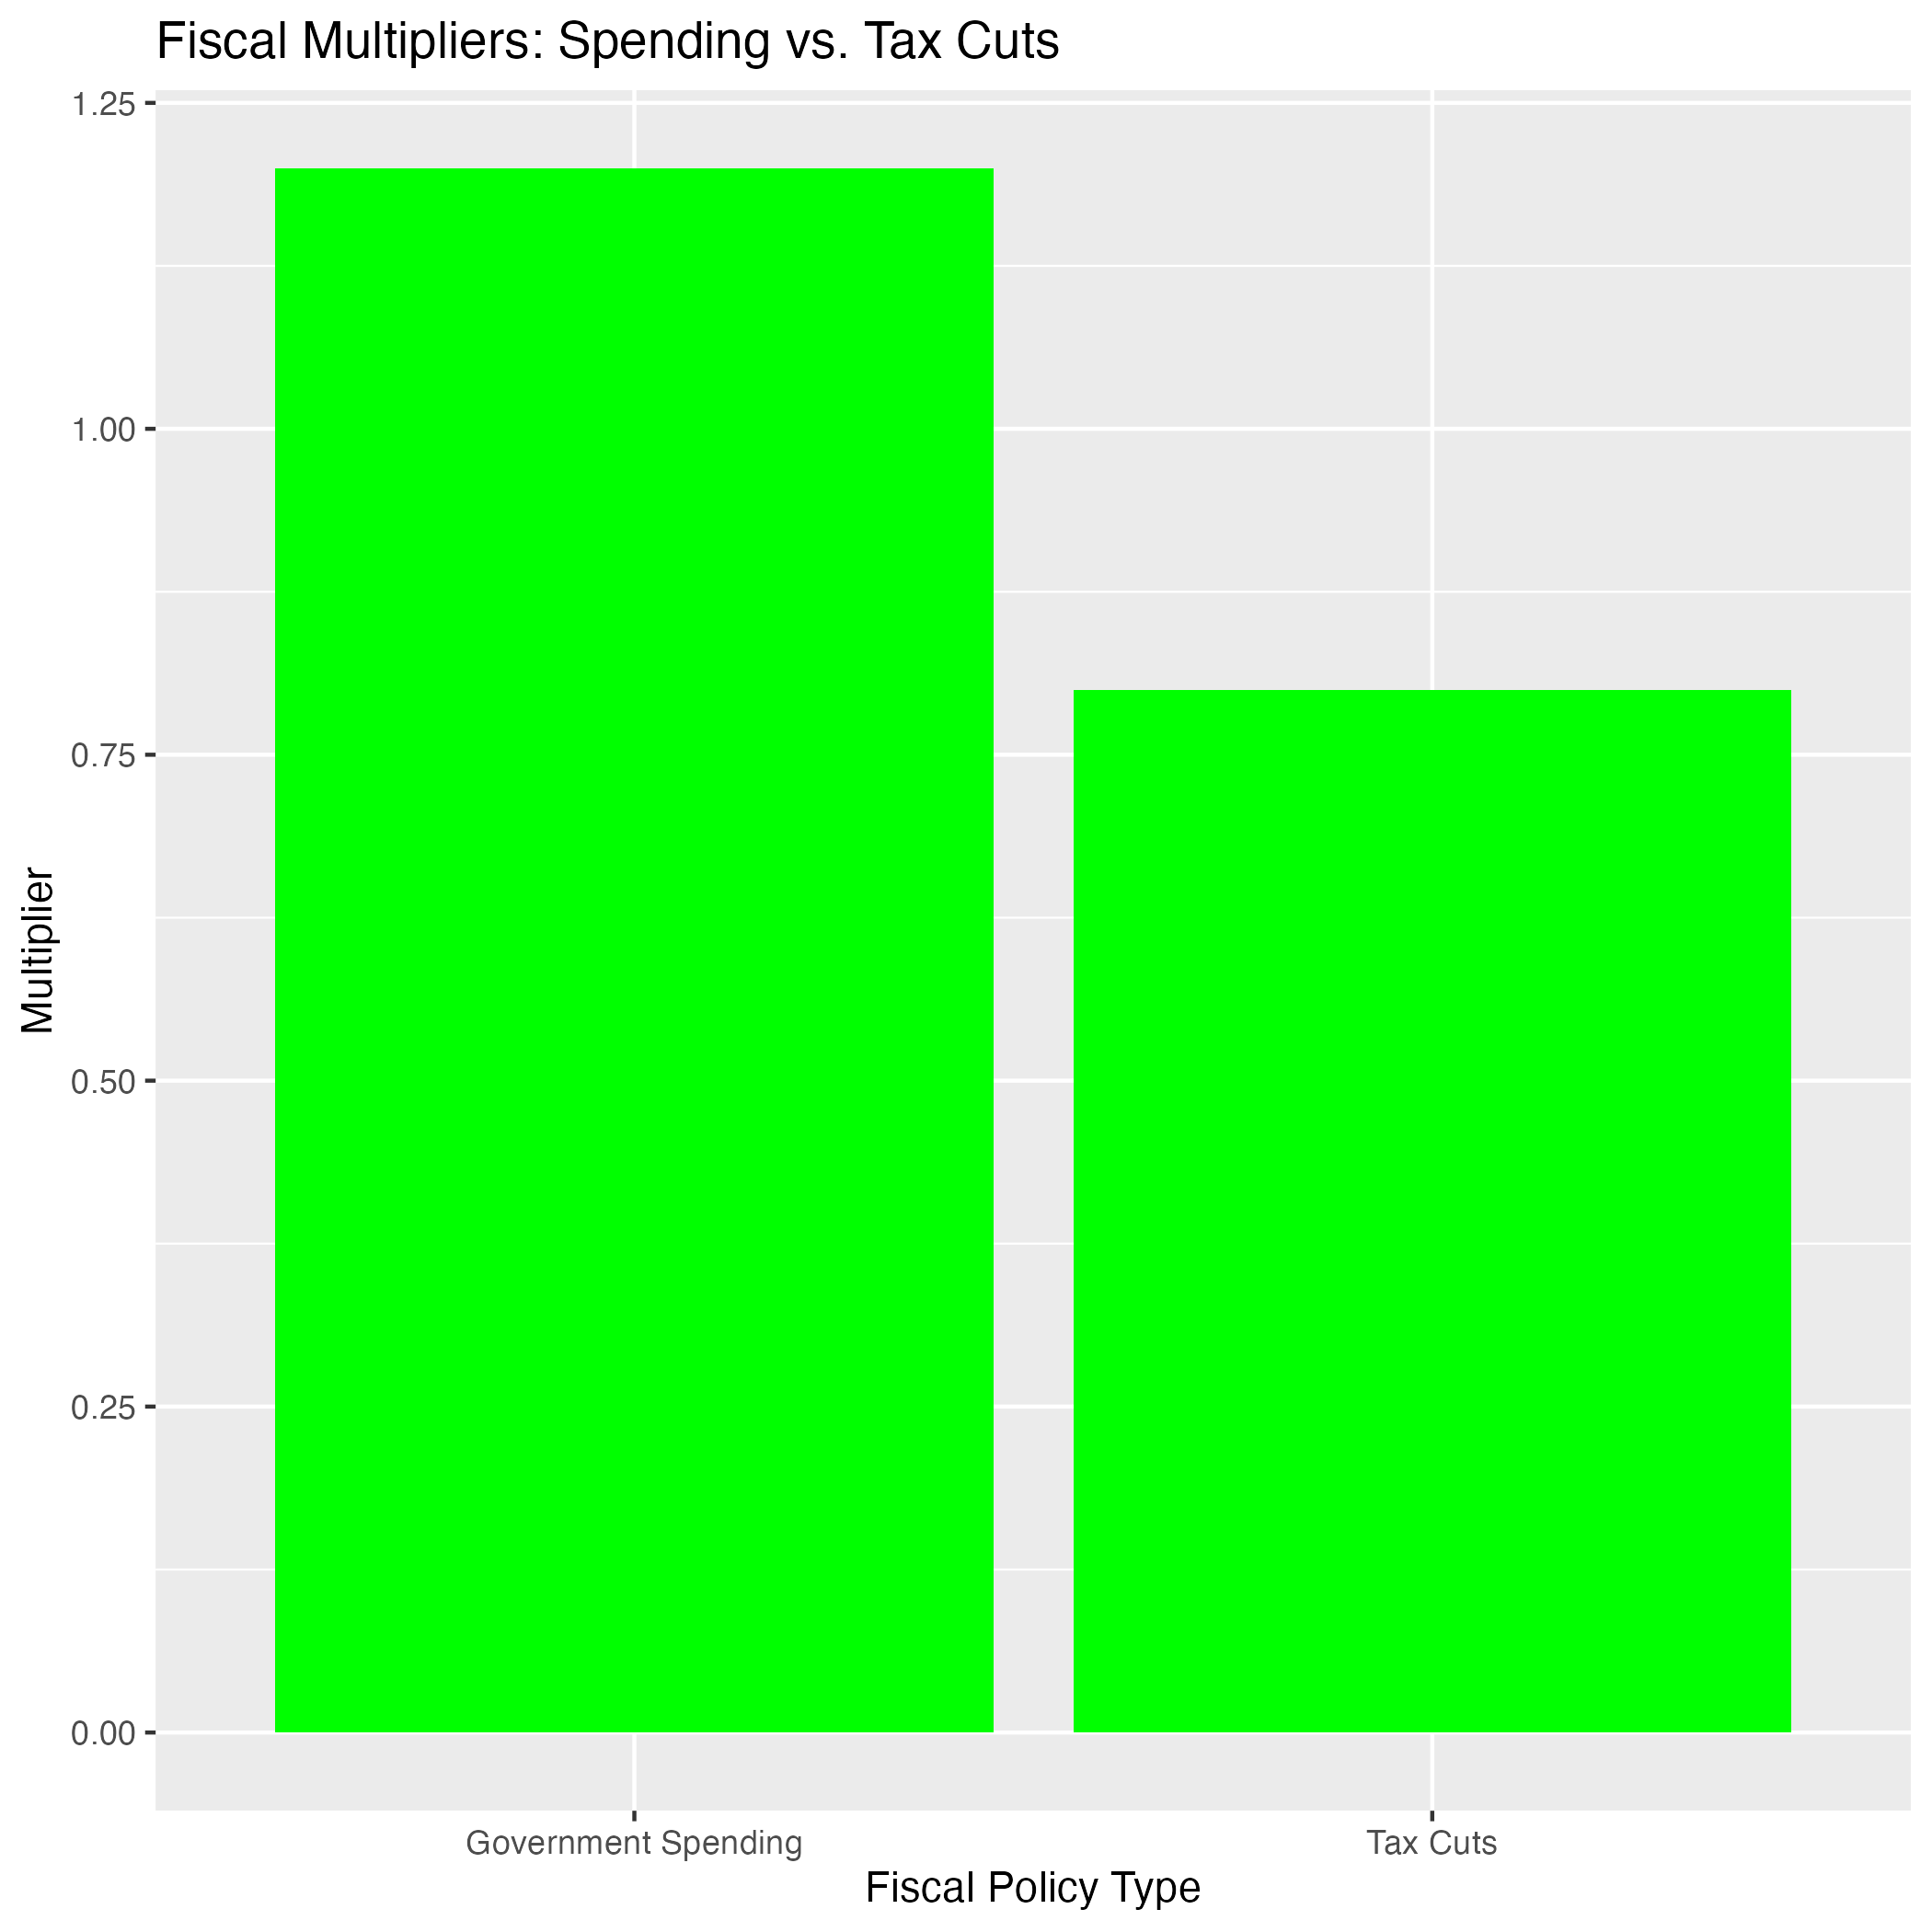
\includegraphics[width=0.8\textwidth]{/Users/cancel/Personal/Coursework/Econ425/VA3/R/Tax_Cuts_Multipliers.png}
        \caption{Fiscal Multipliers: Spending vs. Tax Cuts}
    \end{figure}
\end{frame}

\begin{frame}
    \frametitle{Graph Explanation: Fiscal Multipliers: Spending vs. Tax Cuts}
    This bar plot compares the fiscal multipliers of government spending and tax cuts, showing that government spending generally has a higher multiplier effect, particularly in a recession when there is excess capacity in the economy.
\end{frame}

\begin{frame}
    \frametitle{Key Takeaways: Fiscal Multipliers and Tax Cuts}
    Tax cuts have different effects based on income distribution, with lower-income households more likely to spend additional income. Government spending often has a higher immediate impact on GDP, especially during economic slack.
\end{frame}

\section{VAT Cuts}
\begin{frame}
    \frametitle{VAT Cuts}
    \textbf{Question 6:} Even if not, I heard from a friend, who is a serious economist, that we can always cut the VAT here in the US.

    \textbf{Explanation:} Cutting VAT (Value-Added Tax) can reduce consumer prices and increase consumption. However, it can also reduce government revenue, which might lead to higher deficits if not compensated by other measures. Additionally, VAT cuts can be regressive, benefiting higher-income households more than lower-income ones.

    \textbf{Definition:} VAT is a consumption tax levied on the value added at each stage of production and distribution.

    \textbf{Real-World Example:} The UK temporarily reduced VAT in 2008-2009 to stimulate the economy during the financial crisis.
\end{frame}

\begin{frame}
    \frametitle{Impact of VAT Cuts}
    \begin{figure}[h!]
        \centering
        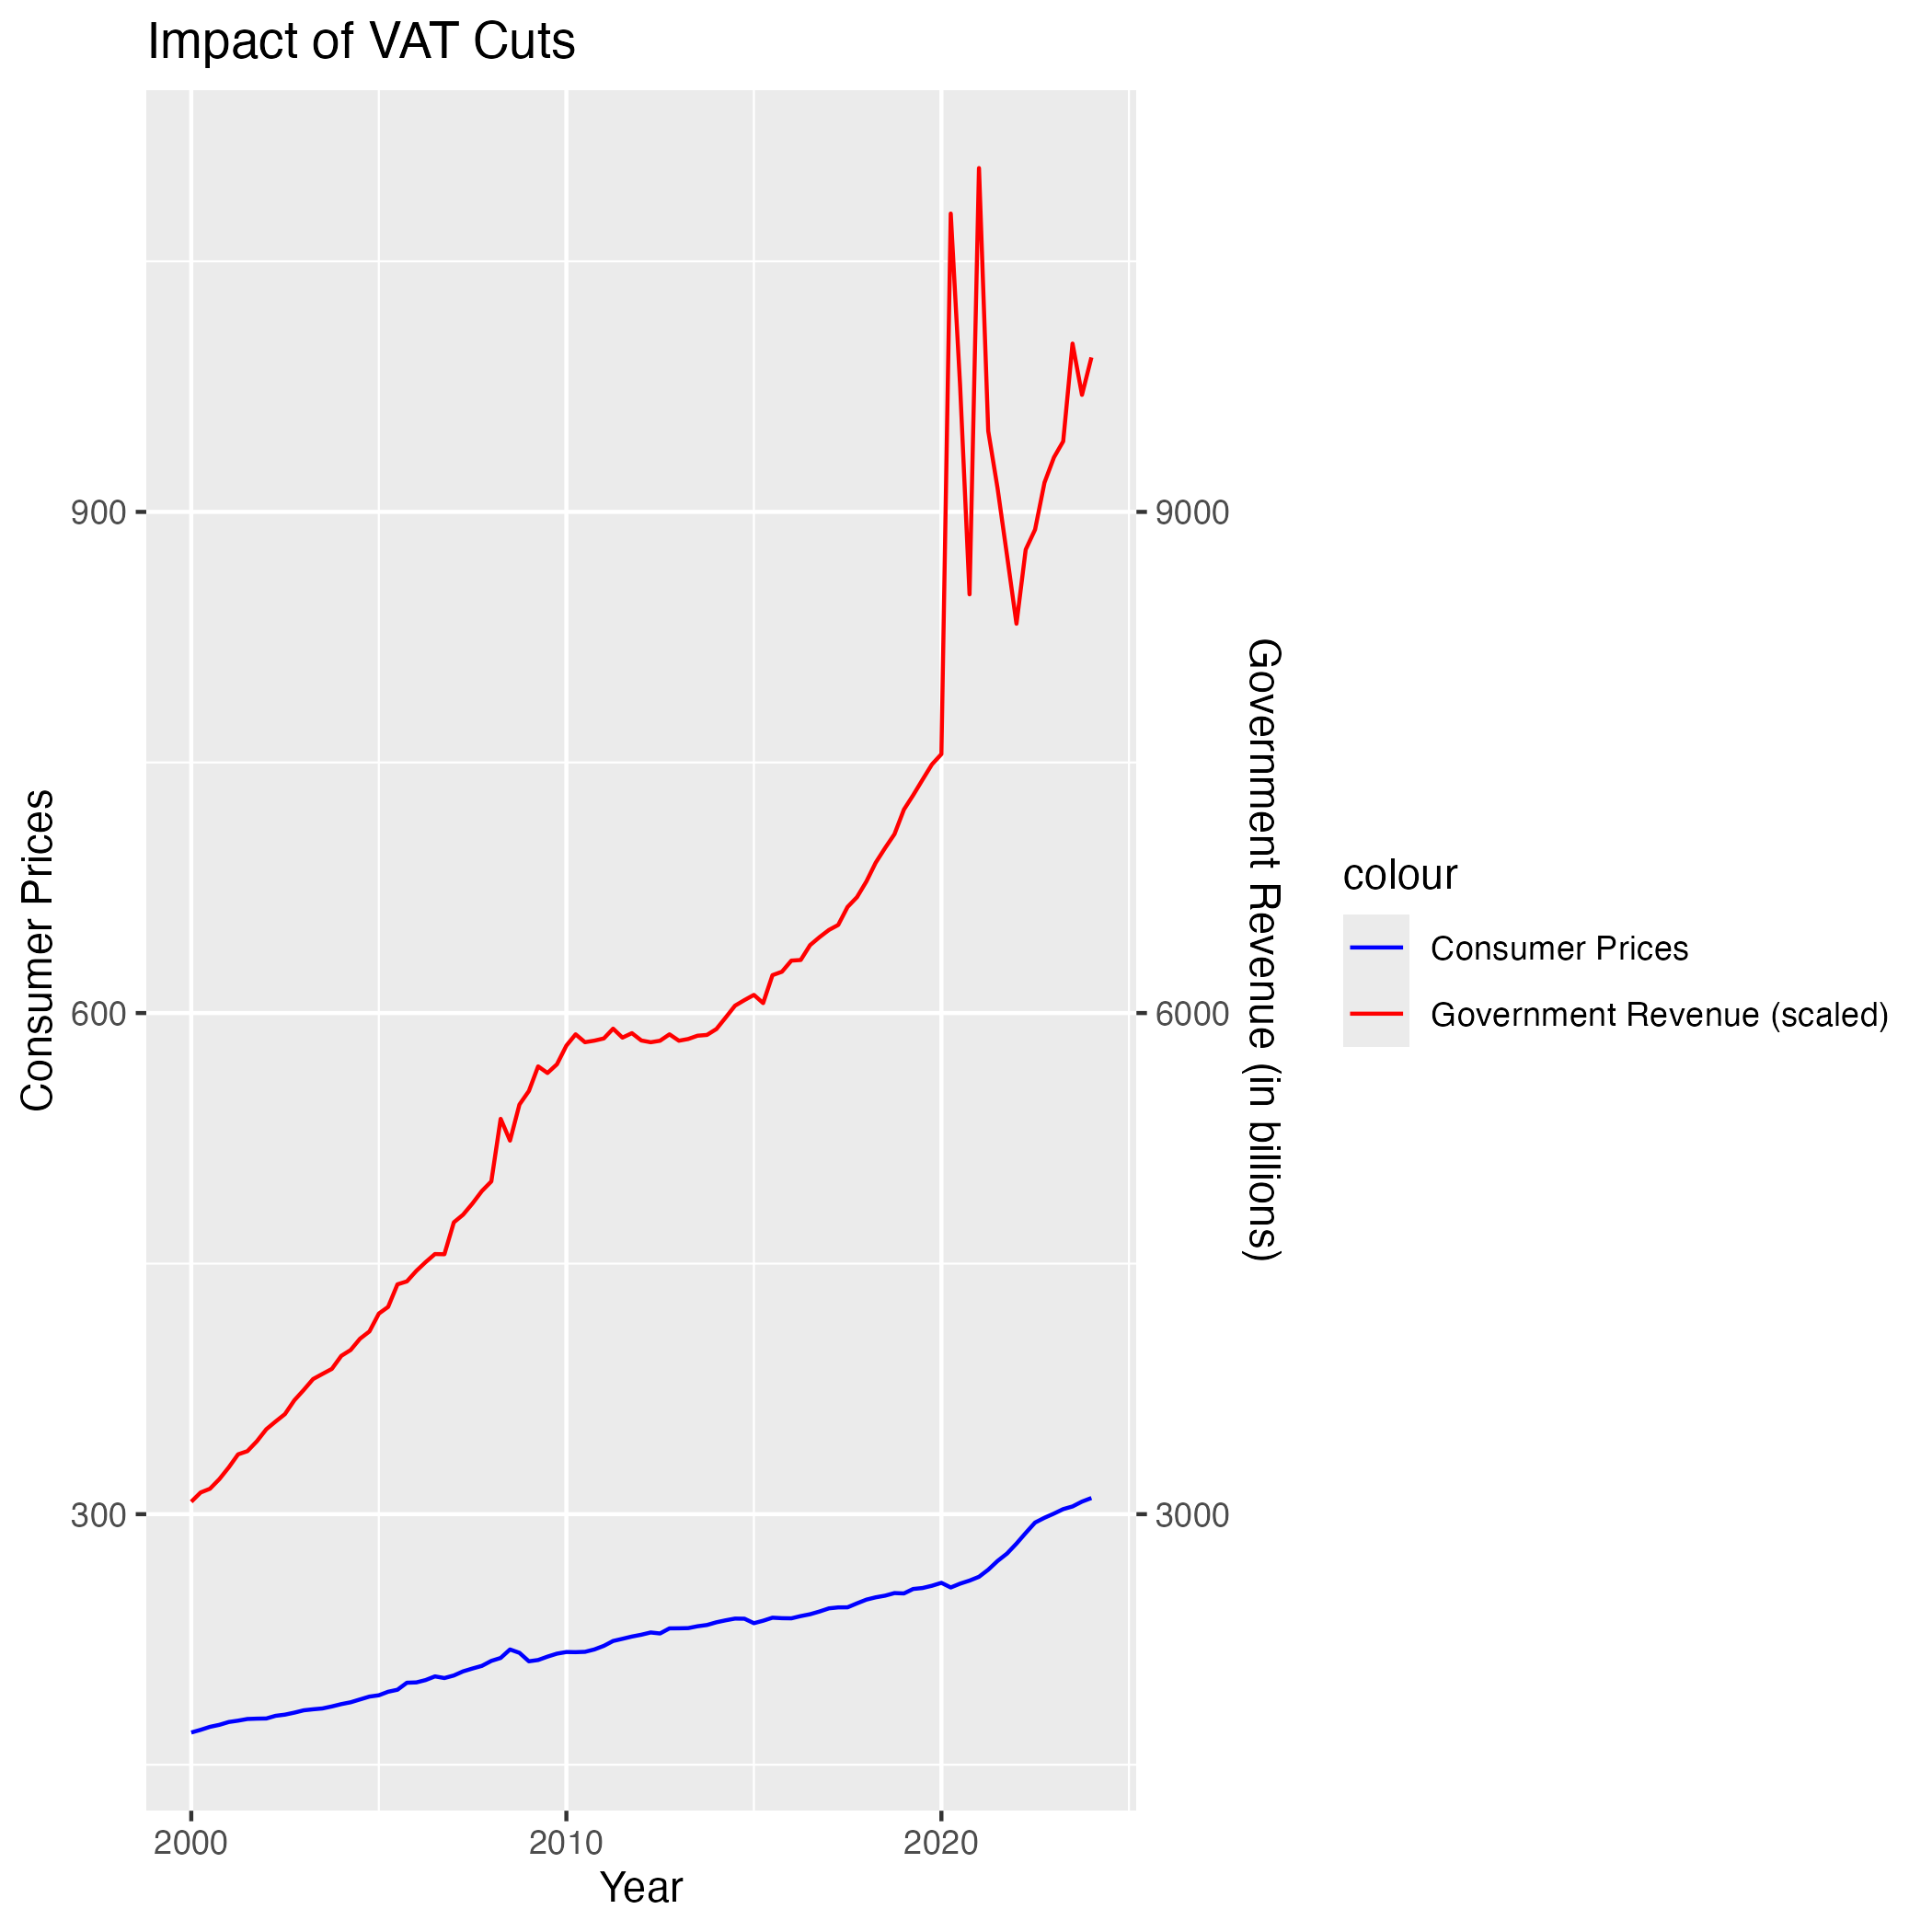
\includegraphics[width=0.8\textwidth]{/Users/cancel/Personal/Coursework/Econ425/VA3/R/VAT_Cuts_Impact.png}
        \caption{Impact of VAT Cuts}
    \end{figure}
\end{frame}

\begin{frame}
    \frametitle{Graph Explanation: Impact of VAT Cuts}
    This dual y-axis plot shows the impact of VAT cuts on consumer prices and government revenue. It highlights how reducing VAT can lower prices but also decrease government revenue, which can affect public services and investments.
\end{frame}

\begin{frame}
    \frametitle{Key Takeaways: VAT Cuts}
    VAT cuts can boost consumption but reduce government revenue. It is important to consider the impact on different income groups and the long-term fiscal health when designing such policies.
\end{frame}

\section{Support for Fiscal Policy}
\begin{frame}
    \frametitle{Support for Fiscal Policy}
    \textbf{Question 7:} Ok, ok. But then, you are probably against fiscal policy as a whole. How can you convince me that you are not just being political?

    \textbf{Explanation:} Fiscal policy is a critical tool for managing the economy. Its effectiveness depends on the context and implementation. Balancing short-term stimulus with long-term sustainability is crucial for economic stability. Fiscal policy can support economic growth through public investments in infrastructure, education, and technology, and can provide social safety nets to reduce inequality and support consumer demand.

    \textbf{Definition:} Fiscal policy involves the use of government spending and taxation to influence the economy.

    \textbf{Real-World Example:} The New Deal programs in the 1930s in the United States used large-scale fiscal interventions to combat the Great Depression.
\end{frame}

\begin{frame}
    \frametitle{Impact of Fiscal Policy on Economic Performance}
    \begin{figure}[h!]
        \centering
        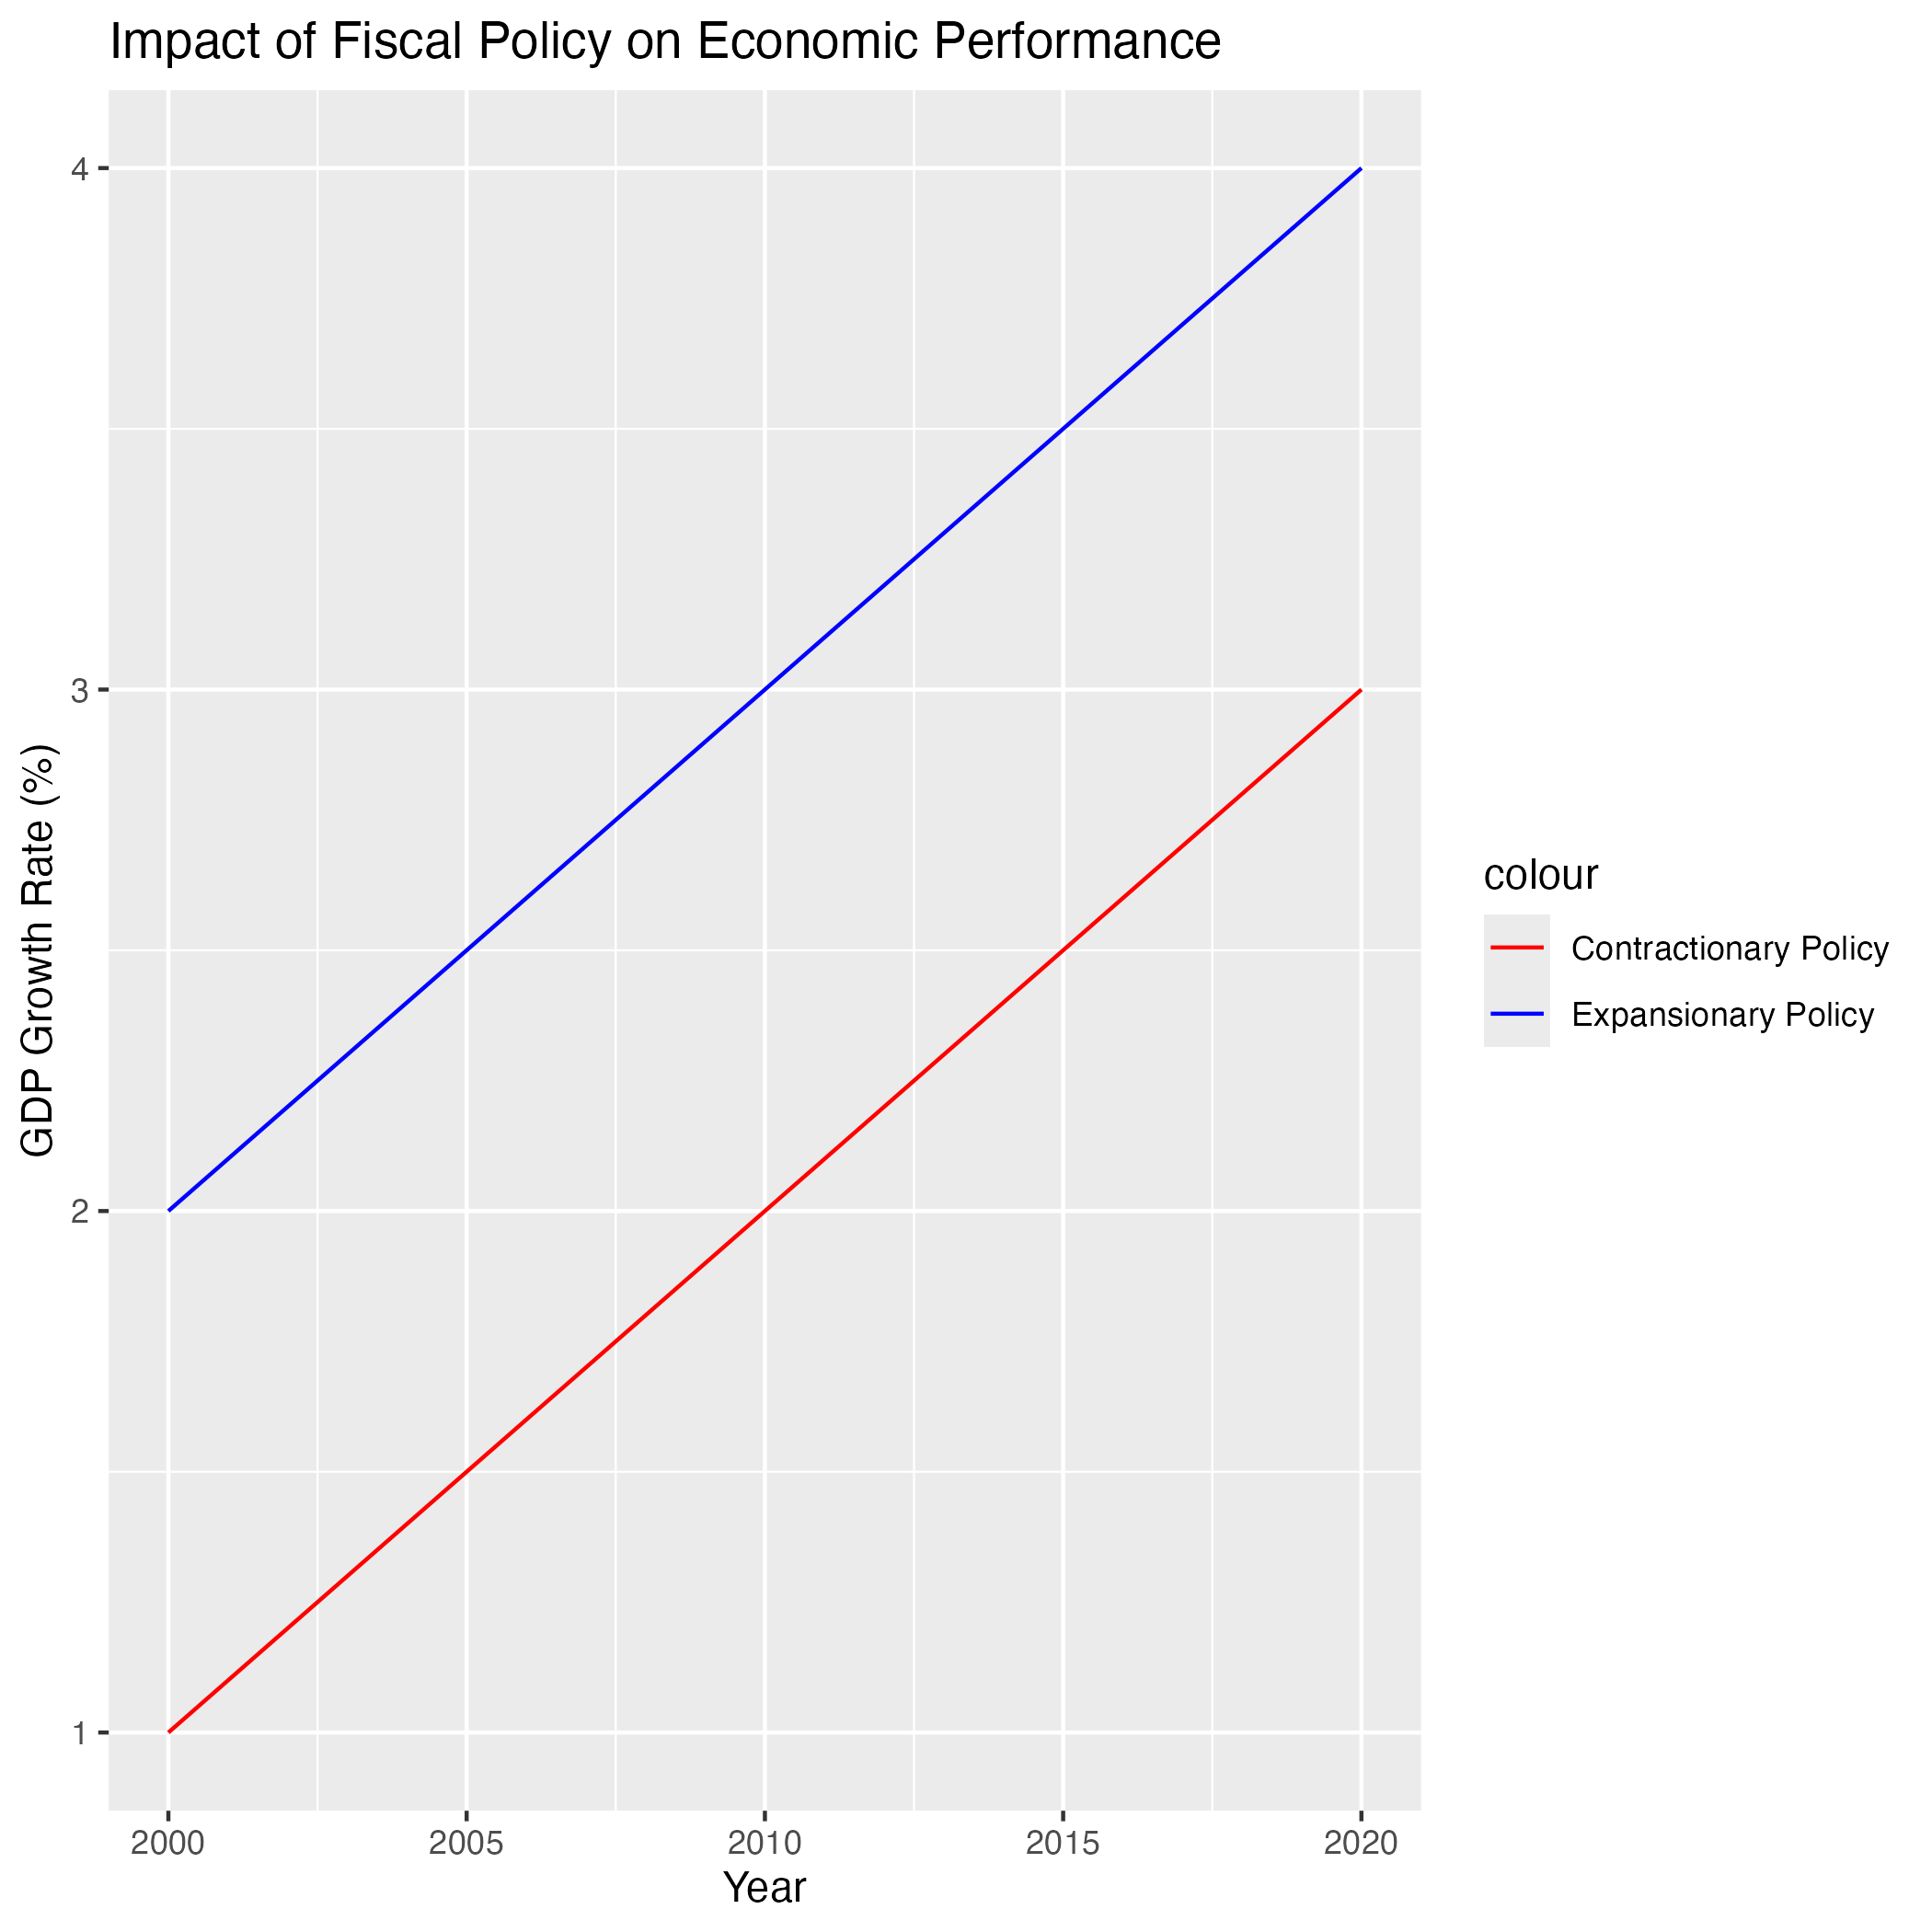
\includegraphics[width=0.8\textwidth]{/Users/cancel/Personal/Coursework/Econ425/VA3/R/Fiscal_Policy_Impact.png}
        \caption{Impact of Fiscal Policy on Economic Performance}
    \end{figure}
\end{frame}

\begin{frame}
    \frametitle{Graph Explanation: Impact of Fiscal Policy on Economic Performance}
    This plot compares economic performance under expansionary and contractionary fiscal policies, showing how different approaches can impact GDP growth rates. It illustrates the importance of context in evaluating the effectiveness of fiscal policy.
\end{frame}

\begin{frame}
    \frametitle{Key Takeaways: Support for Fiscal Policy}
    Fiscal policy is essential for economic stabilization and long-term growth. Public investment can promote economic development, and effective fiscal policy should balance short-term needs with long-term sustainability.
\end{frame}

\section{Conclusion}
\begin{frame}
    \frametitle{Conclusion}
    Thank you for your attention. This concludes my discussion on fiscal policy concepts. If you have any questions, please feel free to ask.
\end{frame}

\end{document}
